\documentclass{standalone}
\usepackage{tikz} % Load TikZ package for drawing

\begin{document}

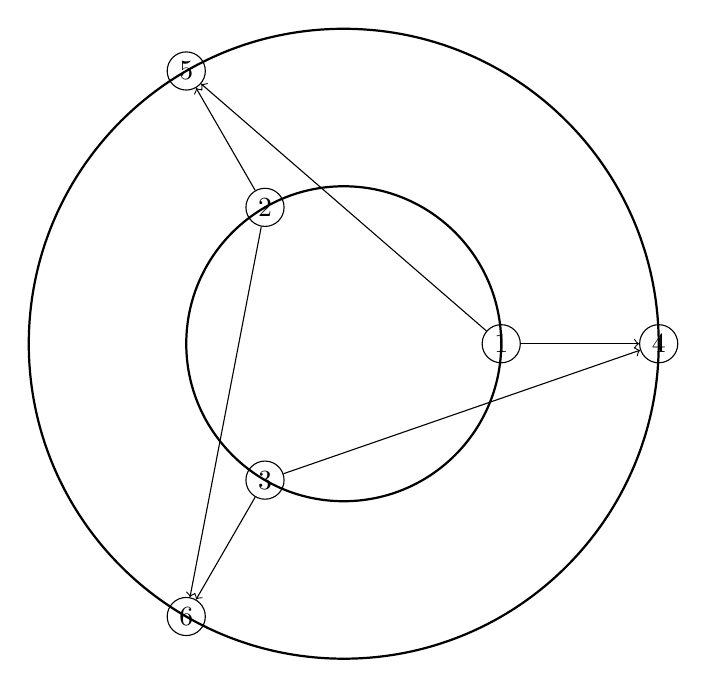
\begin{tikzpicture}
  % Draw the inner concentric circle (radius 2cm)
  \draw[thick] (0,0) circle (2cm);
  % Draw the outer concentic circle (radius 4cm)
  \draw[thick] (0,0) circle (4cm);
  
  % Place nodes on the inner circle (vertices with numbers)
  % Node 1 at 0 degrees (right side of inner circle)
  \node[draw, circle, inner sep=2pt] (inner1) at (0:2cm) {1};
  % Node 2 at 120 degrees (upper left of inner circle)
  \node[draw, circle, inner sep=2pt] (inner2) at (120:2cm) {2};
  % Node 3 at 240 degrees (lower left of inner circle)
  \node[draw, circle, inner sep=2pt] (inner3) at (240:2cm) {3};
  
  % Place nodes on the outer circle (vertices with numbers)
  % Node 4 at 0 degrees (right side of outer circle)
  \node[draw, circle, inner sep=2pt] (outer1) at (0:4cm) {4};
  % Node 5 at 120 degrees (upper left of outer circle)
  \node[draw, circle, inner sep=2pt] (outer2) at (120:4cm) {5};
  % Node 6 at 240 degrees (lower left of outer circle)
  \node[draw, circle, inner sep=2pt] (outer3) at (240:4cm) {6};
  
  % Draw directed edges (arrows) between inner and outer nodes
  % To show dependencies from inner to outer nodes
  \draw[->] (inner1) -- (outer1); % 1 -> 4
  \draw[->] (inner2) -- (outer2); % 2 -> 5
  \draw[->] (inner3) -- (outer3); % 3 -> 6
  % Add cross connections to show more complex dependencies
  \draw[->] (inner1) -- (outer2); % 1 -> 5
  \draw[->] (inner2) -- (outer3); % 2 -> 6
  \draw[->] (inner3) -- (outer1); % 3 -> 4
\end{tikzpicture}

\end{document}